\documentclass[parskip=full,11pt]{scrartcl}
%\usepackage{pdfpages}
\usepackage[utf8]{inputenc}
\usepackage[T1]{fontenc}
\usepackage[german]{babel}
\usepackage[yyyymmdd]{datetime} 
\usepackage{hyperref}
\usepackage[toc, nonumberlist, automake]{glossaries} %added automake option
\usepackage{array,multirow,makecell}

\setcellgapes{1pt}
\makegapedcells
\usepackage[table]{xcolor}
\newcolumntype{V}[1]{>{\centering\arraybackslash }b{#1}}
\newcolumntype{D}[1]{>{\centering\arraybackslash }b{#1}}
\newcolumntype{B}[1]{>{\centering\arraybackslash }b{#1}}
\newcolumntype{A}[1]{>{\centering\arraybackslash }b{#1}}
\usepackage{graphicx}

\usepackage{csquotes}
\usepackage{xcolor}
\usepackage{hyperref}

\definecolor{shadecolor}{RGB}{220,220,220}
\hypersetup{
		pdftitle={Pflichtenheft},
		bookmarks=true,
}
\usepackage{fancyhdr}%<-------------to control headers and footers
\usepackage{tabularx}%<------------- simpler table management
\usepackage{float} 
\usepackage[a4paper,margin=1in,footskip=.25in]{geometry}
\fancyhf{}
\fancyfoot[C]{\thepage} %<----to get page number below text
\pagestyle{fancy} %<-------the page style itself

\title{Pflichtenheft}
\subtitle{Authorisierungsmanagement für eine virtuelle Forschungsumgebung für Geodaten}
\author{Alex\\Anastasia\\Atanas\\Dannie\\ Houra\\Sonya\\}
\date{22.11.17}

% define custom lists
\usepackage{enumitem}

% add glossary
\makeglossaries
\newglossaryentry{V-FOR-WaTer}
{
	name={V-FOR-WaTer},
	description={Virtuelle Forschungsumgebung für die Wasser- und Terrestrische Umweltforschung ist eine generische, virtuelle Forschungsumgebung für den gemeinsamen, systemischen Umgang mit Daten aus der Wasser- und Umweltforschung}, 
}
\newglossaryentry{Benutzer}
{
	name={Benutzer},
	description={Ein Benutzer ist eine Person, die das Portal benutzt. Somit verfügt sie unter anderem über Profilinformationen, die auf dem Datenbank gespeichert sind} 
}
\newglossaryentry{Administrator}
{
	name={Administrator},
description={Ein Administrator ist ein Verwalter des Systems, er unterstützt die Datenbankverwaltung und hat erweiterte Rechte im Vergleich zu Standardbenutzer. Der Administrator ist ein Mitarbeiter von ``V-FOR-WaTer``} 
}
\newglossaryentry{Ressourcenbesitzer}
{
	name={Ressourcenbesitzer},
	description={Ein Ressourcenbesitzer ist ein Benutzer, der eigene Ressourcen erstellt oder Besitzerrechte für Ressourcen von anderen Benutzern bekommen hat}
}
\newglossaryentry{Datenbank}
{
	name={Datenbank},
	description={Eine Datenbank ist eine eine große Menge von Daten, die in einem Computer nach bestimmten Kriterien organisiert sind und komplexe Abfragen zulassen} %todo
}
\newglossaryentry{Loeschrequest}
{
	name={Loeschrequest},
	description={Ein Loeschrequest ist ein Request, der vom Ressourcenbesitzer an Administrator gesendet wird, um Ressourcen aus dem Portal entfernen zu lassen}  %Löschen muss so geschrieben werden, sonst -> Probleme 
}
\newglossaryentry{Web-Portal}
{
	name={Web-Portal},
	description={Ein Web-Portal ist ein Anwendungssystem, das sich durch die Integration von Anwendungen, Prozessen und Diensten auszeichnet. Ein Portal stellt seinem Benutzer verschiedene Funktionen zur Verfügung, wie beispielsweise Navigation und Benutzerverwaltung. Außerdem koordiniert es die Suche und die Präsentation von Informationen und soll die Sicherheit gewährleisten} 
}
\newglossaryentry{Zugriffsrechte}
{
	name={Zugriffsrechte},
	description=
	{Zugriffsrechte sind ein Befugnis den Inhalt einer Ressource zu lesen oder/und auszuführen}
}
\newglossaryentry{Besitzerrechte}
{
	name={Besitzerrechte},
	description=
	{Besitzerrechte sind Rechte, die einem Benutzer Rechteverwaltung und Löschrequestserstellung für eine bestimmte Ressource ermöglichen} 
}
\newglossaryentry{IDs}
{
	name={ID},
	description=
	{Abkürzung für Identifikator. Ein Identifikator (auch Kennzeichen) ist ein mit einer bestimmten Identität verknüpftes Merkmal zur eindeutigen Identifizierung des tragenden Benutzers} 
}
\newglossaryentry{Metadaten}
{
	name={Metadaten},
	description=
	{Metadaten sind Daten, die dazu dienen, Ressource zu beschreiben, ohne ihre Inhalt zu veröffentlichen.} 
}
\newglossaryentry{Zugriffsrequest}
{
	name={Zugriffsrequest},
	description=
	{Ein Zugriffsrequest ist ein Request, das vom Benutzer an den Ressourcenbesitzer gesendet wird, um Befugnis zu erlangen, auf den Inhalt der Ressource zuzugreifen} 
}
\newglossaryentry{Token}
{
	name={Token},
	description=
	{Das Token ist eine Textdatei, die einen Verifizierungsstring enthält. In diesem String sind die ID des Benutzers, seine Rechte auf die Ressourcen im Portal und die Gültigkeitsdauer des Tokens verschlüsselt} 
	plural={Tokens}
}

\def\threedigits#1{%
  \ifnum#1<10 0\fi
  \ifnum#1<1 0\fi
  \number#1}
\begin{document}

\begin{titlepage}
	
	\begin{center}
	{\scshape\LARGE\bfseries Pflichtenheft \par}
	\vspace{1cm}
	{\scshape\Large Praxis der Softwareentwicklung\\}
	\vspace{1cm}
	{\scshape\Large Wintersemester 17/18\\}
	\vspace{3cm}
	{\huge\bfseries Authorisierungsmanagement für eine virtuelle Forschungsumgebung für Geodaten\par}
	\vspace{2cm}
	\vfill
	{\bfseries {\Large Autoren}:\par}
	{\Large Aleksandar Bachvarov}\\
	{\Large Anastasia Slobodyanik}\\
	{\Large Atanas Dimitrov}\\
	{\Large Khalil Sakly}\\
	{\Large Houraalsadat Mortazavi Moshkenan}\\
	{\Large Sonya Voneva}\\
	\vfill
	
	{\large 22.11.17 \par}
	\end{center}
\end{titlepage}
\newpage
\section*{Versionshistorie} 
\begin{tabular}{|V{2cm}|D{3cm}|B{4cm}|A{4cm}}
\hline \rowcolor{lightgray} Version & Datum &  Autor(en) &  Bemerkungen  \\
\hline  1.0 & 8.11.2017 & Houraalsadat Mortazavi Moshkenan & Erstellen \\
\hline  1.1  & 21.11.2017 & Aleksandar Bachvarov, Anastasia Slobodyanik, Atanas Dimitrov, Khalil Sakly, Houraalsadat Mortazavi Moshkenan, Sonya Voneva  & Alle Teile wurden implementiert und Pflichtenheft ist nun Fertig \\
\hline 1.2 & 26.11.2017 & Aleksandar Bachvarov, Anastasia Slobodyanik, Khalil Sakly, Sonya Voneva  & Bemerkungen von der Präsentation hinzufügen  \\
\hline 
\end{tabular}

\newpage
\tableofcontents

\newpage
%\section{Einleitung}
\section{Zielbestimmung}
Das Produkt dient zum Authorisierungsmanagement des \grqq{\gls{V-FOR-WaTer}}\grqq -Web-Portals. Dadurch können die in dem \gls{Web-Portal} registrierten \gls{Benutzer} Zugriffsanfragen für Ressourcen senden, Ressourcen nutzen und Ressourcen selbst erstellen. Dabei dient das Produkt auch zur Unterscheidung zwischen Benutzer, \gls{Ressourcenbesitzer} und \gls{Administrator}.

\subsection{Musskriterien}
Im Folgenden werden Kriterien aufgelistet, die für ein Funktionieren des Produktes unabdingbar sind.

\subsection*{Benutzer}
\begin{itemize}[itemsep=0pt]
\item Der Benutzer kann auf Ressourcen zugreifen, für die er \gls{Zugriffsrechte} hat.
\item Der Benutzer kann dem Ressourcenbesitzer ein \gls{Zugriffsrequest} senden, um Zugriffsrechte zu erlangen.
\item Der Benutzer bekommt Rückmeldung, wenn sein Request erfolgreich gesendet wurde.
\item Der Benutzer bekommt eine E-Mail-Benachrichtigung, wenn seine Zugriffsanfrage genehmigt/abgelehnt wurde.
\item Der Benutzer kann seine eigenen Ressourcen erstellen. Somit wird er der Ressourcenbesitzer dieser Ressourcen.
\item Der Benutzer kann seinen Namen im Portal ändern.
\end{itemize}
 
\subsection*{Ressourcenbesitzer}
\begin{itemize}[itemsep=0pt]

\item Der Ressourcenbesitzer kann Zugriffsrechte für seine eigenen Ressourcen frei oder auf Request vergeben.
\item Der Ressourcenbesitzer kann seine \gls{Besitzerrechte} mit anderen Benutzern teilen.
\item Der Ressourcenbesitzer kann dem Administrator ein \gls{Loeschrequest} senden, um seine eigenen Ressourcen löschen zu lassen.
\item Der Ressourcenbesitzer kann den Namen des Request-Absenders beim Request sehen.
\item Der Ressourcenbesitzer kann seine Ressourcen auf der Profilseite sehen.
\end{itemize}
\newpage

\subsection*{Administrator}
\begin{itemize}[itemsep=0pt]
\item Der Administrator kann Ressourcen löschen.
\item Der Administrator kann Benutzer (vom Portal) entfernen.
\item Der Administrator unterstützt die Datenbankverwaltung.
\item Der Administrator kann Zugriffsrechte für Ressourcen beliebig vergeben (ohne selbst Ressourcenbesitzer zu sein).
\item Der Administrator kann Besitzerrechte für Ressourcen beliebig vergeben (ohne selbst Ressourcenbesitzer zu sein).
\end{itemize}

\subsection{Wunschkriterien}
Im Folgenden werden Kriterien aufgelistet, die das Produkt umsetzen kann.
Im Verlauf des Entwurfs wird entschieden, welche der Kriterien  implementiert werden können.
\begin{itemize}[itemsep=0pt]
\item Wird eine Ressource gelöscht, so werden alle Besitzer per E-Mail benachrichtigt. 
\item Eine Zugriffsanfrage kann für mehrere Ressourcen gleichzeitig gesendet werden.
\item Der Benutzer kann dem Administrator ein Request für Administratorrechte senden.
\item Dem Benutzer stehen Hilfeverweise zur Verfügung.
\item Zur Verifizierung von Rechten werden \glspl{Token} implementiert.
\item Mehrmaliges Versagen eines Requests führt zur Benachrichtigung des Administrators.
\item Der Ressourcenbesitzer kann Zugriffsrechte für seine eigenen Ressourcen an eine Gruppe von Benutzern vergeben.
\item Der Administrator kann einen Benutzer blockieren.
\item Der Administrator kann Benutzer anhand von Vorname und/oder Nachname suchen.
\end{itemize}
\newpage


\subsection{Abgrenzungskriterien}
Im Folgenden wird beschrieben, was das Produkt explizit nicht leisten soll.
\begin{itemize}[itemsep=0pt]
\item Das Produkt dient nicht zur Authentifizierung.
\item Das Produkt dient nicht zur Kommunikation zwischen Benutzern.
\item Das Produkt unterstützt keine mobile Version.
\item Die \glspl{IDs} von Benutzern sind weder sichtbar noch veränderbar.
\item Die E-Mail-Adressen von Benutzern sind nicht veränderbar.
\item Das Produkt steht nicht zur Verfügung für Benutzer ohne Account.
\end{itemize}

\section{Produkteinsatz}
Das Produkt wird in die Virtuelle Forschungsumgebung (VFU) für die Wasser-
und Terrestrische Umweltforschung (\grqq{\gls{V-FOR-WaTer}}\grqq) im Rahmen des Netzwerks
Wasserforschung Baden-Württemberg eingesetzt. Die VFU legt ihre Schwerpunkte
auf die Datenhaltung und den direkten Zugriff auf Analysewerkzeuge für Daten
aus der Wasser- und Umweltforschung. Das Produkt dient der
Rechteverwaltung für diese Daten.

\subsection{Anwendungsbereiche}
\begin{itemize}[itemsep=0pt]
\item Umweltforschung
\item Datenhaltung
\end{itemize}

\subsection{Zielgruppen}
\begin{itemize}[itemsep=0pt]
\item Administrator(en) des Portals %(Mitarbeiter von V-FOR-WaTer)
\item Wissenschaftliche Mitarbeiter von \grqq{\gls{V-FOR-WaTer}}\grqq
\item Externe Benutzer des Portals
\end{itemize}
\newpage
\subsection{Betriebsbedingungen}
\begin{itemize}[itemsep=0pt]
\item Einsatz in einem Webportal mit einer \gls{Datenbank}.
\item Das Produkt benötigt eine funktionierende Internetverbindung.
\item Die Betriebsdauer ist täglich 24 Stunden.
\end{itemize}


\section{Produktumgebung}
Das Produkt wird in die virtuelle Forschungsumgebung für Wasser- und Terrestrische Umweltforschung \grqq{\gls{V-FOR-WaTer}}\grqq \: integriert.\\
Das Produkt ist weitergehend unabhängig vom Betriebssystem, sofern folgende Produktumgebung vorhanden ist:

\subsection{Software}
\begin{itemize}[itemsep=0pt]
\item Serverseite:
	\begin{itemize}
	\item Webserver Apache 
	\item SQLite–Datenbank
	\end{itemize}
\item Clientseite:
	\begin{itemize}
	\item Moderne Webbrowser:
		\begin{itemize}
		\item Chrome
		\item Firefox
		\item Safari
		\item Microsoft Edge
		\end{itemize}
	
	\end{itemize}
\end{itemize}
\newpage
\subsection{Hardware}
\begin{itemize}[itemsep=0pt]

	\item Serverseite:
	\begin{itemize}
	\item Netzwerkfähig
	\item Rechner, der die Ansprüche der o.g. Server-Software erfüllt.
	\end{itemize}
	\item Clientseite:
	\begin{itemize}
	\item Standardrechner
	\item Internetverbindung
	\end{itemize}
\end{itemize}
\section{Funktionale Anforderungen}
Im Folgenden werden die funktionalen Anforderungen (sowohl Musskriterien als auch Wunschkriterien) erläutert. Die optionalen Funktionalitäten, die sich aus den Wunschkriterien ergeben, sind \colorbox{shadecolor}{farblich gekennzeichnet}.
\subsection{Benutzerfunktionen}
\begin{enumerate}[label={\textbf{/F\protect\threedigits{\theenumi}0/}}, leftmargin=*]
\item \label{FAB1} \textbf{Profilübersicht:} \\ Der angemeldete Benutzer kann seine personenbezogenen Daten (Name, Vorname) auf seiner Profilseite sehen.\\\\\
\textbf{Beschreibung:}\\
\begin{enumerate}[label=(\arabic*), leftmargin=*]
\item Nach dem Anmelden kann der Benutzer seine Profilseite öffnen.
\item Auf der Profilseite werden personenbezogenen Daten des Benutzers angezeigt.
\end{enumerate}

\item \label{FAB2} \textbf{Datenänderung:} \\ Der angemeldete Benutzer kann seinen Namen ändern.\\\\
\textbf{Beschreibung:}\\
\begin{enumerate}[label=(\arabic*), leftmargin=*]
\item Nach dem Öffnen seiner Profilseite kann der Benutzer den Edit-Button rechts von seinem Namen klicken.
\item Der Benutzer kann im Eingabefeld seinen Namen ändern und durch Klicken des Save-Buttons das Ergebnis speichern.
\item  Nach dem Speichern wird der geänderte Name auf der Profilseite angezeigt.
\end{enumerate}

\item \label{FAB3} \textbf{Ressourcenzugriff:} \\Der angemeldete Benutzer kann auf Ressourcen zugreifen, für die er Zugriffsrechte hat.
\\ Von Ressourcen, für die der Benutzer keine Rechte hat, sind nur die Metadaten sichtbar.\\\\
\textbf{Beschreibung:}\\
\begin{enumerate}[label=(\arabic*), leftmargin=*]
\item Der angemeldete Benutzer kann eine Ressourcenliste auf Ressourcenübersichtseite sehen.
\item Der Benutzer kann Inhalt der Ressourcen, für die er Zugriffsrechte hat, durch Klicken des Buttons \grqq{Zugreifen}\grqq \: ansehen.
\item Der Benutzer kann von Ressourcen, für die er keine Zugriffsrechte hat, ausschließlich Metadaten sehen.
\end{enumerate}

\item \label{FAB4} \textbf{Ressourcenerstellung:}\\ Der Benutzer kann neue Ressourcen hochladen.\\\\
\textbf{Beschreibung:}\\
\begin{enumerate}[label=(\arabic*), leftmargin=*]
\item Der angemeldete Benutzer kann auf seiner Profilseite im Abschnitt \grqq{Meine Ressourcen}\grqq \: den Button \grqq{Hinzufügen}\grqq \: klicken.
\item Im geöffneten Dialog kann der Benutzer eine Datei zum Hochladen auswählen.
\item Nach dem Hochladen der Datei kann der Benutzer den Namen der Ressource eingeben und die Ressource speichern.  
\end{enumerate}

\item \label{FAB5} \textbf{Zugriffsrechte für Ressourcen anfordern:}\\ Der Benutzer kann Requests an den Ressourcenbesitzer senden, um die Zugriffsrechte für gewünschte Ressourcen zu erlangen.\\\\
\textbf{Beschreibung:}\\
\begin{enumerate}[label=(\arabic*), leftmargin=*]
\item Der angemeldete Benutzer kann Ressourcen auf der Ressourcenübersichtseite sehen.
\item Der Benutzer kann durch Klicken des Buttons \grqq{Request}\grqq \: Zugriffsrechte für Ressourcen anfordern.
\item Der Benutzer kann im Dialogfenster das Absenden der Requests bestätigen oder ablehnen.
\item Durch Klicken des ``Absenden``-Buttons wird ein Request erstellt und der Ressourcenbesitzer per E-Mail benachrichtigt.
\item Nach dem erfolgreichen Absenden des Zugriffsrequests wird  \grqq{Request}\grqq -Button durch ``Stornieren``-Button ersetzt.
\end{enumerate}
\newpage

\item \label{FAB6} \textbf{Benachrichtigung:}\\ Der Benutzer wird per E-Mail benachrichtigt, wenn sein Request abgelehnt/genehmigt wird.\\\\
\textbf{Beschreibung:}\\
\begin{enumerate}[label=(\arabic*), leftmargin=*]
\item Zugriffrequests vom Benutzer werden vom Ressourcenbesitzer bearbeitet.
\item Nachdem Zugriffsrequest genehmigt oder abgelehnt wird, wird der Benutzer per E-Mail darüber benachrichtigt.
\end{enumerate} 

\item \label{FAB7} \colorbox{shadecolor} {\textbf{Requestsübersicht:}}\\ Der angemeldete Benutzer kann seine abgesendeten Requests auf seiner Profilseite sehen. \\\\
\textbf{Beschreibung:}\\
\begin{enumerate}[label=(\arabic*), leftmargin=*]
\item Abgesendete und noch nicht bearbeitete Requests des Benutzers werden auf seiner Profilseite im Abschnitt \grqq{Abgesendete Requests}\grqq \: aufgelistet.
\item Nachdem Request bearbeitet wird, wird es aus Requestsliste gelöscht.
\end{enumerate}

\item \label{FAB8} \colorbox{shadecolor} {\textbf{Multiple Request:}}\\ Der Benutzer kann Zugriffsrequest für mehrere Ressourcen gleichzeitig senden.\\\\
\textbf{Beschreibung:}\\
\begin{enumerate}[label=(\arabic*), leftmargin=*]
\item Der Benutzer kann mehrere Ressourcen auf der Ressourcenübersichtseite auswählen.
\item Durch Klicken des \grqq{Request}\grqq -Buttons werden Requests an den Besitzer abgesendet.
\end{enumerate}

\item \label{FAB9} \colorbox{shadecolor} {\textbf{Administratorrechte anfordern:}}\\ Der Benutzer kann ein Request an Administrator senden, um Administratorrechte zu erlangen.\\\\
\textbf{Beschreibung:}\\
\begin{enumerate}[label=(\arabic*), leftmargin=*]
\item Der Benutzer kann durch Klicken des \grqq{Admin werden}\grqq -Buttons Administratorrechte anfordern.
\item Die Administratoren werden per E-Mail darüber benachrichtigt.
\end{enumerate}
\newpage

\item \label{FAB10} \colorbox{shadecolor}{\textbf{Erstellung von Tokens}}\\ Der Benutzer bekommt ein Token, mit dem er seine Rechte für Ressourcen auf einem externen Webserver verifizieren kann.\\\\
\textbf{Beschreibung:}\\
\begin{enumerate}[label=(\arabic*), leftmargin=*]
\item Ein Token wird bei einer Veränderung der Benutzerrechte erstellt bzw. aktualiesiert und dem Benutzer gesendet. 
\item Immer wenn der Benutzer eine externe Webseite besucht, die Ressourcen von \grqq{\gls{V-FOR-WaTer}}\grqq \: verwaltet, wird sein Token für eine leichtere Autorisierung benutzt. 

\end{enumerate}
\end{enumerate}
\subsection{Administratorfunktionen}
\begin{enumerate}[label={\textbf{/F\protect\threedigits{\theenumi}0/}}, leftmargin=*, resume]
\item \label{FAA1}\textbf{Bearbeiten von Loeschrequest}\\ Der Administrator erhält von einem Ressourcenbesitzer ein Request zum Löschen von Ressourcen.\\\\
\textbf{Beschreibung:}\\
\begin{enumerate}[label=(\arabic*), leftmargin=*]
\item Nachdem der Ressourcenbesitzer ein Loeschrequest gesendet hat, werden alle Administratoren durch eine E-Mail benachrichtigt.
\item Die Nachricht enthält die Daten des Ressourcenbesitzers und den Namen der zu löschenden Ressource.
\item Der Administrator kann seine Entscheidung direkt durch ein Interface (zwei Buttons \grqq{Ja}\grqq  \: oder \grqq{Nein}\grqq  \:) am Nachrichtbildschirm treffen.
\item Nachdem der Administrator den ``Ja``-Button klickt, kann er das Löschen von Ressourcen im Dialogfenster bestätigen oder ablehnen.  
\end{enumerate}


\item \label{FAA2} \textbf{Löschen von Ressourcen}\\ Der Administrator kann die Ressourcen im Portal löschen.\\\\
\textbf{Beschreibung:}\\
\begin{itemize}[itemsep=0pt, leftmargin=*]
\item Das Löschen kann entweder auf die in \ref{FAA1} beschriebene Weise oder auch ohne Request geschehen.
\end{itemize}

\newpage
\item \label{FAA3} \textbf{Rechte gewähren}\\ Der Administrator kann einem Benutzer Zugriffs- oder Besitzerrechte gewähren und wieder entziehen.\\\\
\textbf{Beschreibung:}\\
\begin{enumerate}[label=(\arabic*), leftmargin=*]
	\item Der Administrator kann Zugriffs- oder Besitzerrechte für jede Ressource an andere Benutzer vergeben.
	\item Alle Rechte können von dem Administrator entzogen werden.
	\end{enumerate}

\item \label{FAA4} \textbf{Benutzer löschen}\\ Der Administrator kann einen Benutzer löschen.\\\\
\textbf{Beschreibung:}\\
\begin{enumerate}[label=(\arabic*), leftmargin=*]
	\item Zusammen mit dem Account werden die personenbezogenen Daten des Benutzers entfernt.
	\item Der Administrator kann des gelöschten Benutzers Account und Daten nicht wiederherstellen. Der Benutzer muss sich erneut registrieren.
	\end{enumerate}

\item \label{FAA5} \colorbox{shadecolor} {\textbf{Bearbeiten von Adminrequest}}\\ Der Administrator bekommt Request von einem Benutzer, der vom Administratorrechte verlangt.\\\\
\textbf{Beschreibung:}\\
\begin{enumerate}[label=(\arabic*), leftmargin=*]
	\item Der Administrator kann Adminrequest ablehnen oder genehmigen.
	\item Nach der Bearbeitung vom Request wird der entsprechende Benutzer per E-Mail benachrichtigt.
	\end{enumerate}

\item \label{FAA6} \colorbox{shadecolor} {\textbf{Benutzer blockieren}}\\ Der Administrator kann einen Benutzer blockieren, damit dieser sich nicht anmelden kann.\\\\
\textbf{Beschreibung:}\\
\begin{enumerate}[label=(\arabic*), leftmargin=*]
	\item Das Blockieren führt nicht zur Löschung von Account oder Daten.\\
		Nach dem Blockieren kann der Benutzer sich nicht mehr anmelden.
	\item Der Administrator kann den blockierten Benutzer wieder zum Anmelden zulassen.
	\end{enumerate}
\newpage

\item \label{FAA7} \colorbox{shadecolor} {\textbf{Benutzer suchen}}\\  Administratoren können Benutzer anhand von Vorname und Nachname suchen.\\\\
\textbf{Beschreibung:}\\
\begin{enumerate}[label=(\arabic*), leftmargin=*]
	\item Der Administrator kann den Namen des Benutzers in das Suchfeld eingeben.\\
	\item Treffer werden im Ergebnisbereich angezeigt.
	\end{enumerate}
\end{enumerate}

\subsection{Ressourcenbesitzerfunktionen}
\begin{enumerate}[label={\textbf{/F\protect\threedigits{\theenumi}0/}}, leftmargin=*, resume]
\item \label{FARB1} \textbf{Übersicht der Requests:}\\
Eine Liste von Requests ist auf Profilseite einzusehen.\\\\
\textbf{Beschreibung:}\\
\begin{enumerate}[label=(\arabic*), leftmargin=*]
\item Nach der Anmeldung wird dem Ressourcenbesitzer eine Liste von Requests, die von anderen Benutzern gesendet wurden, angezeigt.
\item Nach der Bearbeitung eines Requests, wird dieses aus der Liste gelöscht.  
\end{enumerate}

\item \label{FARB2} \textbf{Übersicht der Ressourcen:}\\
Es steht eine Liste von Ressourcen, für die der Benutzer Besitzerrechte hat,  auf der Profilseite zur Verfügung.\\\\
\textbf{Beschreibung:}\\
\begin{enumerate}[label=(\arabic*), leftmargin=*]
\item Die vom Benutzer erstellten Ressourcen werden auf seiner Profilseite angezeigt, solange er die Besitzerrechte für diese hat.
\item Die Ressourcen, für die der Benutzer Besitzerrechte bekommen hat, werden ebenso auf seiner Profilseite angezeigt.  
\end{enumerate}


\item \label{FARB3} \textbf {Vergabe der Zugriffsrechte:}\\ 
Der Besitzer kann Zugriffsrechte ohne Request an andere Benutzer vergeben.\\\\
\textbf{Beschreibung:}\\
\begin{itemize}[itemsep=0pt, leftmargin=*]
\item Der Ressourcenbesitzer kann in seiner Profilseite für eine bestimmte Ressource durch Klicken des \grqq{Zugriffsrechte vergeben}\grqq -Buttons Zugriffsrechte an andere Benutzer vergeben.
\end{itemize}
\newpage

\item \label{FARB4} \textbf {Request auf Zugriffsrechte ablehnen/genehmigen:}\\ 
Der Ressourcenbesitzer bekommt von anderen Benutzern Zugriffsrequest. \\\\
\textbf{Beschreibung:}\\
\begin{enumerate}[label=(\arabic*), leftmargin=*]
\item Der Ressourcenbesitzer kann Requests, mit welchen andere Benutzer Zugriffsrechte anfordern, entweder ablehnen oder annehmen.
\item In beiden Fälle (Genehmigung/Ablehnung) wird der entsprechende Benutzer benachrichtigt.
\item Im Falle der Genehmigung bekommt der Benutzer die Zugriffsrechte auf  gewünschte Ressourcen.
\end{enumerate}

\item \label{FARB5} \textbf{Vergabe der Besitzerrechte:}\\
Der Ressourcenbesitzer kann seine Besitzerrechte mit anderen Benutzern teilen.\\\\
\textbf{Beschreibung:}\\
\begin{enumerate}[label=(\arabic*), leftmargin=*]
\item Der Ressourcenbesitzer kann Besitzerrechte mit anderen Benutzern teilen, indem er den \grqq{Besitzerrechte teilen}\grqq -Button der entsprechenden Ressource klickt.
\item Dieser Vorgang kann beliebig oft wiederholt werden.
\end{enumerate}

\item \label{FARB6} \textbf{Loeschrequest senden:}\\
Der Ressourcenbesitzer kann zum Löschen seiner eigenen Ressourcen dem Administrator ein Loeschrequest senden.\\\\
\textbf{Beschreibung:}\\
\begin{enumerate}[label=(\arabic*), leftmargin=*]
\item Der Ressourcenbesitzer kann dem Administrator ein Loeschrequest senden, um seine eigene Ressource löschen zu lassen, indem er den \grqq{Löschrequest senden}\grqq -Button der entsprechenden Ressource klickt.
\item Wird diese Ressource gelöscht, bekommt der Ressourcenbesitzer eine E-Mail-Benach-
richtigung.
\end{enumerate}

\item \label{FARB7} \colorbox{shadecolor} {\textbf{Löschbenachrichtigungen:}}\\
Beim Löschen einer Ressource werden alle Ressourcenbesitzer benachrichtigt.\\\\
\textbf{Beschreibung:}\\
\begin{itemize}[itemsep=0pt, leftmargin=*]
\item Wird eine Ressource vom Administrator gelöscht, werden alle Ressourcenbesitzer per E-Mail benachrichtigt.
\end{itemize}

\newpage
\item \label{FARB8} \colorbox{shadecolor} {\textbf{Zugriffsrechte an eine Gruppe vergeben:}}\\
Der Ressourcenbesitzer kann Zugriffsrechte für seine eigenen Ressourcen an eine Gruppe von Benutzern vergeben.\\\\
\textbf{Beschreibung:}\\
\begin{enumerate}[label=(\arabic*), leftmargin=*]
\item Die Vergabe von Zugriffsrechten kann entweder auf die in \ref{FARB3} und \ref{FARB4} beschriebene Weise einzeln oder kumulativ geschehen.
\end{enumerate}

\end{enumerate}


\section{Produktdaten}
\subsection{Benutzerdaten}
\begin{enumerate}[label={\textbf{/D\protect\threedigits{\theenumi}0/}}, leftmargin=*]
     		\item Vorname
     		\item Nachname
     		\item ID
     		\item E-Mail Adresse 
\end{enumerate}
     		 
\subsection{Sonstiges}
\begin{enumerate}[label={\textbf{/D\protect\threedigits{\theenumi}0/}}, leftmargin=*, resume]
		\item Ressourcenliste, die der Benutzer besitzt
        	\item Status (Administrator, Benutzer)     
\end{enumerate}


\subsection{Ressourcendaten}
\begin{enumerate}[label={\textbf{/D\protect\threedigits{\theenumi}0/}}, leftmargin=*, resume]
		\item Titel
		\item Erstellungsdatum
		\item Besitzer
        	\item Leser     
\end{enumerate}

\newpage
\section{Nichtfunktionale Anforderungen}
\begin{enumerate}[label={\textbf{/NF\protect\threedigits{\theenumi}0/}}, leftmargin=*]
\item Eine Änderung von Rechten wird nach nächster Seitenaktualisierung sichtbar.
\item Zur Erstellung eines Requests sind maximal 5 Schritte nötig.
\item Zur Erstellung einer neuen Ressource sind maximal 5 Schritte nötig.
\item Eine Änderung von Rechten führt nicht zur Veränderung von Ressourcen.
\item Verständlichkeit des Produkts wird durch ausreichende Hilfeverweise gewährleistet.
\item Effiziente Nutzung des Produkts soll durch angemessenes Zeitverhalten garantiert werden.  
\end{enumerate}

\section{Systemmodelle}

\subsection{Szenarien}
\subsubsection*{Einfache Benutzerfunktionen}
Alice ist seit kurzem verheiratet und möchte darum ihren Nachnamen im Portal von \grqq{\gls{V-FOR-WaTer}}\grqq \: ändern. Sie loggt sich im System ein und sieht ihr Profil. Dann klickt sie den Button \grqq{Name editieren}\grqq \: und tippt ihren neuen Namen ein. 

Nun möchte sie eine neue Ressource erstellen, darum klickt sie den Button \grqq{Ressource  hinzufügen}\grqq. Später entscheidet sich Alice ihre neue Ressource X zu überprüfen. Sie sucht im Portal nach der Ressource X und findet sie. Weil sie die Besitzerin ist, kann sie X zugreifen.\\

	\begin{center}
	\includegraphics[width=0.6\textwidth]{Szenario_1.png}
	\end{center}
\newpage
\subsubsection*{Zugriffsrequest senden}
Bob hat Interesse an einer Ressource X im Portal von \grqq{\gls{V-FOR-WaTer}}\grqq. Er probiert den Inhalt von X zuzugreifen. Leider hat er keine Zugriffsrechte dafür. Um solche Rechte zu bekommen, soll er ein Request am Besitzer von X senden, in diesem Fall - Alice. Bob wählt die Option \grqq{Zugriffsrechte anfragen}\grqq. 

Nach wenigen Sekunden bekommt Alice eine E-Mail-Benachrichtigung über das neue Request. Um zu entscheiden, ob sie die Zugriffsanfrage genehmigt, loggt sie sich im Portal ein. Dann sieht sie Bobs Anfrage und beschließt sie zu genehmigen. In kurzem bekommt Bob eine E-Mail mit der guten Neuigkeit. Nun kann er die Ressource zugreifen und ist glücklich.\\
	
	\begin{center}
	\includegraphics[width=1\textwidth]{Szenario_2.png}
	\end{center}

\newpage
\subsubsection*{Besitzerrechte teilen}
Der Besitzer der Ressource Y, nämlich Bob, ist ein sehr beschäftigter Mann. Er hat keine Zeit und Lust jeden Tag die zahlreiche Zugriffsanfragen für Rechte auf Y zu beantworten. Deshalb hat er sich entschieden seine Besitzerrechte mit drei seinen Mitarbeitern zu teilen. \\
Er findet die Ressource Y und wählt die Option \grqq{Besitzerrechte teilen}\grqq. Dann findet er seine Mitarbeiter durch ihre Namen. Auf diese Weise kann jeder von der neuentstandene Gruppe von Besitzern eine zukünftige Zugriffsanfrage genehmigen oder ablehnen.\\

	\begin{center}
	\includegraphics[width=0.7\textwidth]{Szenario_3bevor.png}
	
	\includegraphics[width=0.7\textwidth]{Szenario_3nach.png}
	\end{center}

\subsubsection*{Ressource editieren}
Alice hat ihre Meinung geändert und möchte jetzt etwas in Ressource X korrigieren. Da das Portal diese Option nicht anbietet, muss sie zuerst erneut die Ressource X erstellen. Dieses mal beinhaltet X aber auch die gemachte Korrektur. Danach sendet sie ein Loeschrequest am Administrator, damit er die alte Version von X zerstört.\\
	
	\begin{center}
	\includegraphics[width=1\textwidth]{Szenario_4.png}
	\end{center}
	
\subsection{Diagramme}

\subsubsection*{Funktionenübersichtsdiagramm}

	\begin{center}
	\includegraphics[width=0.95\textwidth]{Funktionen_uebersicht.png}
	\end{center}
	
\subsubsection*{Kontrollflussdiagramm \grqq{Ressource zugreifen}\grqq}

	\begin{center}
	\includegraphics[width=1\textwidth]{Kontrollfluss.png}
	\end{center}
	
\subsubsection*{Zustandsdiagramm \grqq{Zugriffsrequest}\grqq}
Das Diagramm stellt die mögliche Zustände eines Zugriffsrequests dar.
\\

	\begin{center}
	\includegraphics[width=0.9\textwidth]{Zustandsdiagramm.png}
	\end{center}
	\newpage
\subsection{Benutzerschnittstelle}
Im Folgenden werden Benutzerschnittstelle-Skizzen abgebildet. Skizzen stellen ein mögliches Aussehen des Produkts dar. Weitere Änderungen während Entwicklung und nach Auftraggeberanfrage sind möglich.
\subsubsection*{Profilseite von Benutzer}
Der Benutzer sieht auf seiner Profilseite seinen Namen und hat die Möglichkeit ihn zu ändern. Außerdem sieht er Requests- und Ressourcenbereiche, die leer sind, solange er keine Ressourcen besitzt, bzw. keine Requests bekommen hat. Der Benutzer hat jedoch die Möglichkeit eigene Ressourcen hinzuzufügen.
	\begin{center}
	\includegraphics[width=0.9\textwidth]{Profilseite_Benutzer.png}
	\end{center}
\newpage
\subsubsection*{Profilseite von Ressourcenbesitzer}

Links auf seiner Profilseite sieht der Ressourcenbesitzer einen Block mit den offenen Requeste, die er bearbeiten soll/kann (durch Klicken eines der beiden Buttons mit den Symbolen für ``genehmigen`` und ``ablehnen``). Dabei sind die Absender des Requests und die gewünschte Ressource zu sehen. Alle Requeste sind vom Typ ``Zugriffsrequest``. Im rechten Block hat der Ressourcenbesitzer die Möglichkeit neue Ressource zu erstellen. Folgende Optionen stehen dem Besitzer zur Verfüging:
\begin{itemize}
	\item Zugriff auf eigene Ressource 
	\item Änderung der Zugriffs-/Besitzerrechte 
	\item Erstellung des Löschrequests für seine Ressource
\end{itemize} 

	\begin{center}
	\includegraphics[width=0.9\textwidth]{Profilseite_Besitzer.png}
	\end{center}
\newpage	
\subsubsection*{Profilseite von Administrator}
Die Profilseite eines Administrators ist eine Erweiterung der Profilseite des Benutzers. Zusätzlich hat der Administrator die Option Ressourcen zu löschen. Im ``Requests``-Block werden die o.g. ``Löschrequeste`` aufgelistet. Der Administrator kann diese Requests bearbeiten, indem er einen der beiden Buttons für Genehmigen und Ablehnen klickt.
	\begin{center}
	\includegraphics[width=0.9\textwidth]{Profilseite_Admin.png}
	\end{center}
\newpage	
\subsubsection*{Administratorseite}
Der Administrator sieht einen zusätzlichen ``Admin``-Button im obenstehenden Menu. Durch Klicken dieses Buttons wird die Administratorseite geöffnet. Auf Administratorseite hat der Administrator die Möglichkeit die im Portal registrierten Benutzer, sowie alle Ressourcen zu verwalten. Bezüglich der Benutzer hat er folgende Optionen:
\begin{itemize}
	\item Zugriffsrechte korrigieren (umfasst vergeben und entziehen)
	\item Besitzerrechte korrigieren (umfasst vergeben und entziehen)
	\item Benutzer blockieren
	\item Benutzer löschen (die persönliche Daten des Benutzers werden vom System gelöscht, ausschließlich seiner Ressourcen)
\end{itemize}  
 Im Block ``Ressourcenübersicht`` kann der Administrator:
 \begin{itemize}
 	\item Alle Ressourcen zugreifen, unabhängig davon, ob er der Besitzer ist
 	\item Einem Benutzer Zugriffs-/Besitzerrechte auf eine bestimmte Ressource vergeben
 	\item Einem Benutzer Zugriffs-/Besitzerrechte auf eine bestimmte Ressource entziehen
 	\item Eine beliebige Ressource löschen
 \end{itemize}
	\begin{center}
	\includegraphics[width=0.9\textwidth]{Adminseite.png}
	\end{center}
	
\subsubsection*{Ressourcensuche}
Die ``Ressourcensuche``-Seite ist für jeden im Portal registrierten Benutzer zugänglich. Im Menu auf linker Seite kann man Suchkrieterien ändern. Nach dem Klicken des ``Zeige gewählte Datensätze``-Buttons werden die Ergebnisse im zentralen Block unter “Ressourcenübersicht” aufgelistet. Für die ``public`` Ressourcen oder für diejenige, für die der Benutzer Zugriffsrechte hat, sieht er einen Button ``Zugreifen``. Für die ``geschlossene`` (d.h. zu denen er keinen Zugang hat) kann der Benutzer ein Zugriffsrequest dem Ressourcenbesitzer senden, indem er den ``Request``-Button klickt. Wurde das Request abgesendet und noch nicht bearbeitet, so ist der ``Request``-Button nicht klickbar.
	\begin{center}
	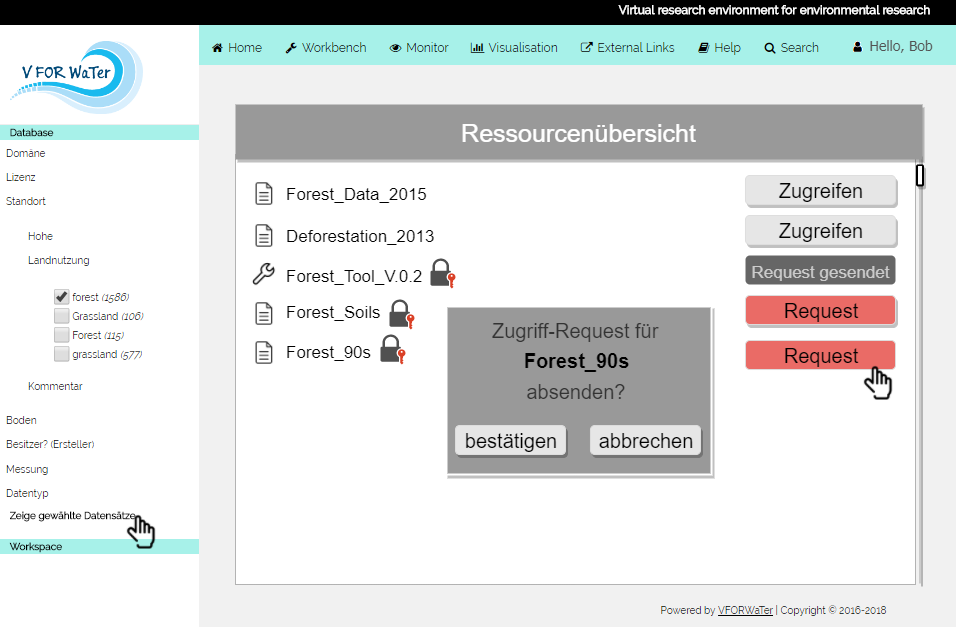
\includegraphics[width=0.9\textwidth]{Ressourcensuche.png}
	\end{center}
	
	
\section{Qualitätsbestimmungen}

\renewcommand{\arraystretch}{1.5}
\begin{table}[H]
  \begin{center}
    \begin{tabularx}{\textwidth}{X c c c c}
      \hline
      
      \textbf{{\large Produktivität}} & \textbf{{\large sehr wichtig}} & \textbf{{\large wichtig}} & \textbf{{\large normal} } &\textbf{{\large nicht relevant }}\\
      
      \hline      
      \multicolumn{5}{l}{\textbf{Funktionalität}}\\      
      \hline      
      Angemessenheit &   & x &   &  \\
	  Richtigkeit & x &   &   &  \\
	  Interoperabilität & x &   &   &  \\
      Sicherheit &   & x &   &  \\	
		    
	  \hline	  
      \multicolumn{5}{l}{\textbf{Zuverlässigkeit}}\\     
      \hline
      Reife &   &   & x &  \\
	  Fehlertoleranz &   &   &   & x\\
	  Wiederherstellbarkeit &   &   &   & x\\
		
	  \hline	  	
	  \multicolumn{5}{l}{\textbf{Benutzbarkeit}}\\
      \hline
      Verständlichkeit & x &   &   &  \\
	  Erlernbarkeit &   & x &   &  \\
	  Bedienbarkeit & x &   &   &  \\
	  
	  \hline	  	
	  \multicolumn{5}{l}{\textbf{Effizienz}}\\
      \hline
      Zeitverhalten &   &   & x &  \\
	  Verbrauchsverhalten & x &   &   &  \\	
	  
	  \hline	  	
	  \multicolumn{5}{l}{\textbf{Änderbarkeit}}\\
      \hline
      Analysierbarkeit &   &   &   & x\\
	  Modifizierbarkeit & x &   &   &  \\
	  Stabilität &   & x &   &  \\
	  Prüfbarkeit &  & x &  & \\

	  
	  \hline	  	
	  \multicolumn{5}{l}{\textbf{Benutzbarkeit}}\\
      \hline
      Anpassbarkeit & x &  &  & \\
	  Installierbarkeit &  & x &  & \\
	  Konformität &  &  &  & x\\
	  Austauschbarkeit & x &  &  & \\
	  
	  \hline      			
    \end{tabularx}
  \end{center}
  
\end{table}
\renewcommand{\arraystretch}{1}

\section{Globale Testfälle}
\subsection{Benutzertestfälle}
\begin{enumerate}[label={\textbf{/T\protect\threedigits{\theenumi}0/}}, leftmargin=*]
\item Profilseite öffnen. (\ref{FAB1})
\item Namen ändern. (\ref{FAB2})
\item Ressourcen öffnen. (\ref{FAB3})
\item Neue Ressource erstellen. (\ref{FAB4})
\item Request senden. (\ref{FAB5})
\item Benachrichtigungen kontrollieren. (\ref{FAB6})
\item Requestliste ansehen. (\ref{FAB7})
\item Multiple Request senden. (\ref{FAB8})
\item Administratorrechte anfragen. (\ref{FAB9})
\item Token erstellen und validieren. (\ref{FAB10})
\end{enumerate}

\subsection{Administratortestfälle}
\begin{enumerate}[label={\textbf{/T\protect\threedigits{\theenumi}0/}}, leftmargin=*, resume]
\item Löschrequest ablehnen. (\ref{FAA1})
\item Löschrequest genehmigen. (\ref{FAA1})
\item Ressource löschen. (\ref{FAA2})
\item Zugriffsrechte einem Benutzer geben.(\ref{FAA3})
\item Zugriffsrechte von einem Benutzer entziehen.(\ref{FAA3})
\item Leserechte zu einem Benutzer geben.(\ref{FAA3})
\item Leserechte von einem Benutzer entziehen.(\ref{FAA3})
\item Account und Daten eines Benutzers löschen.(\ref{FAA4})
\item Adminrequest ablehnen. (\ref{FAA5})
\item Adminrequest genehmigen. (\ref{FAA5})
\item Nach einem Benutzer suchen und ihn blockieren . (\ref{FAA6},\ref{FAA7})
\end{enumerate}

\subsection{Ressourcenbesitzertestfälle}
\begin{enumerate}[label={\textbf{/T\protect\threedigits{\theenumi}0/}}, leftmargin=*, resume]
\item Requestsliste kontrollieren.(\ref{FARB1})
\item Liste von eigenen Ressourcen kontrollieren.(\ref{FARB2})  %todo
\item Zugriffsrechte an anderen Benutzer vergeben.(\ref{FARB3})
\item Request auf Zugriffsrechte ablehnen.(\ref{FARB4})
\item Request auf Zugriffsrechte genehmigen.(\ref{FARB4})
\item Besitzerrechte an anderen Benutzer vergeben.(\ref{FARB5})
\item Löschrequest absenden.(\ref{FARB6})
\item Löschbenachrichtigung kontrollieren.(\ref{FARB7})
\item Zugriffsrechte an eine Gruppe von Benutzern vergeben.(\ref{FARB8}) 
\end{enumerate}
\newpage
\setglossarystyle{altlist}
\printglossary	
\glsaddall
\end{document}
\grid
\grid
